\section{Исследование и построение решения задачи}

\label{subsec:androidoverview}\subsection{Обзор архитектуры Android}

\subsubsection{Программный Стек}
\label{androidDesc}

ОС Android -- широко распространённая платформа на рынке мобильных
устройств. Здесь рассматривается программный стек Android, т.е. уровни
ОС, предоставляющие интерфейсы одним компонентам системы и использующие
возможности других. Android работает на базе распространённой ОС Linux, 
ядро Android по сути является ядром Linux с небольшими изменениями и
оптимизациями. Это значит, что большинство классических функций
операционных систем (такие как файловые системы, планирование процессов,
управление памятью) в Android реализуется также, как в Linux. 

\begin{figure}
\centering
\subfloat{\label{fig:android_arch}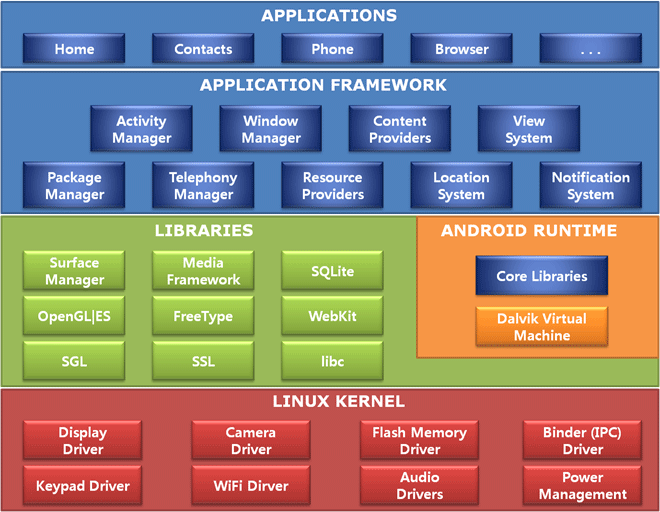
\includegraphics[width=140mm]{external/typical-schematic-of-android_structure.png}} 
\caption{Иллюстрация программного стека Android}
\end{figure}

Далее рассмотрим основные уровни программного стека Android,
изображённые на рисунке \ref{fig:android_arch}:

\textbf{Приложения} : пользовательские приложения, написанные на java,
распространяемые через AndroidMarket или через APK-файлы. Сюда можно
отнести почтовые клиенты, браузеры, медиа-проигрователи и другие
приложения, которыми пользователь обычно пользуется непосредственно
взаимодействуя с ними. 

\textbf{Фреймворк уровня приложений} : набор java классов и пакетов,
предоставляющих API для написания приложений. Набор предоставляемой
функциональности довольно широк: от управления жизненным циклом
приложения до элементов пользовательского интерфейса. Здесь же
предоставляются интерфейсы для взаимодействия приложений друг с другом,
использования одним приложением функций другого.

\textbf{Системные библиотеки} : Набор c/c++ библиотек, применяемых для
написания приложений в Android. Доступны приложениям через фреймворк.
Данные библиотеки реализуют различные ресурсоёмкие задачи, решение
которых посредством java-библиотек вылилось бы в проблемы с
производительностью. В набор входят библиотеки для работы с различными
медиа-форматами (png, jpg, mp3, H.264 и другие), базами данных (sqlite), 
шрифтами, стандартная библиотека с/c++ (Android использует собственную
вариацию под названием bionic), opengl для рисование графики, webkit для
написания web-браузеров. 

\textbf{Android Runtime} : Android использует собственную java-машину
Dalvik Virtual Machine для исполнения java-приложений. DVM используется
из соображений ограниченного объёма памяти на мобильных устройствах. Для
эффективной реализации sandbox-ов для приложений, сущности DVM
запускаются специальным процессом zygote. Также на этом уровне находятся
различные системные сервисы и демоны, работающие с ядром ОС,
устройствами и т.д., например vold, adbd, usbd.

\textbf{Ядро Linux} : В Android используется частично изменённая версия
ядра Linux (обычно используются стабильные ветки ядра 2.6),
оптимизированная под специфику мобильных устройств. Здесь реализуются
драйвера различных физических устройств, системы контроля доступа,
алгоритмы управления виртуальной памятью, файловые системы, сетевой
стек.

В данной работе нас будет интересовать именно ядро Linux. Рассмотрим в
следующем разделе изменения, которые вносит Android в ядро Linux, и на
корелляцию между версиями Linux в Android и в ОС GNU/Linux.

\subsubsection{Сравнения ядер Android и GNU/Linux}

Ядро Linux подходит для использования на самых разных платформах:
встроенные системы, реального времени, высоконагруженные системы и
обычные персональные компьютеры. Когда Linux адаптировался для Android
пришлось вносить изменения в ядро для оптимизации некоторых аспектов
межпроцессного взаимодействия, а также делать поправки на особенности
загрузки ОС на разных устройствах.

Android активно используют передачу данных между процессами, а также
даёт возможность процессам организовать свои процедуры RPC (Remote
Procedure Call). Стандартные средства IPC Linux недостаточно эффективны
для обработки частых запросов на передачу данных, поэтому в Android
появляется существует собственный механизм IPC - Binder. Данный
компонент состоит из нескольких частей: драйвер ядра, реализующий
эффективную передачу данных через общее для всех процессов пространство
ядра, и подсистема рантайма, которая обрабатывает все запросы процессов
на IPC и выполняет их на уровне системных вызовов (взаимодействие с
драйвером).

Система ashmem разделяемой памяти вводит несколько иной, более
эффективный на мобильных устройствах подход, чем классический POSIX SHM.
Вместо файлового API, ashmem позволяет выделять участки разделяемой
памяти с использованием системного вызова mmap, с аргументом файловым
дескриптором, открытым на специальном устройстве /dev/ashmem. Так ashmem
способен отслеживать все области разделяемой памяти в системе, и
уничтожать неиспользуемые в случае нехватки памяти.

В числе прочих изменений, внесённых разработчиками Android можно
упомянуть pmem, аллокатор физической памяти, разделяемой между кодом
ядра и пользовательского пространства, logger реализующий общий
интерфейс логгирования для всех процессов, файловая система yaffs2,
различные патчи, уменьшающие потребление электроэнергии и ещё несколько
архитектурно-зависимых изменений.

По ситуации на март 2014 года, в проекте SEAndroid ядро соответствует 
версии 3.4 обычного ядра Linux.

\subsection{Построение решения}

Рассмотрим возможности для построения системы динамической смены
контекстов безопасности в Android. Для реализации данной задачи
потребуется использовать некоторую систему, позволяющую в зависимости от
внутреннего состояния программы изменять контекст безопасности.
Очевидно, что данная система должна действовать централизованно для всех
приложений в системе, её действия должны быть прозрачны для исполняемого
пользовательского кода. Поэтому предлагается инструментировать
виртуальное адресное пространство приложения контрольными точками, при
попадании исполнения на которые система будет выполнять смену контекста.
Предлагается проводить данную инструментацию при старте приложения из
ядра ОС. На данный момент ОС Android не предоставляет возможности для
динамической инструментации приложения точками останова, но как было
замечено в разделе \ref{subsec:androidoverview} Android использует в
качестве ядра Linux, а значит имеет смысл перенести имеющуюся в Linux
систему динамической инструментации uprobes. 

\subsubsection{uprobes}

Фреймворк динамической инструментации кода приложений точками останова
uprobes используется в системном профилировщике perf для сборки
различной информации по используемым в приложении аппаратным ресурсам,
таким как количество затраченных тактов процессора, количество промахов
кэша при обращении к памяти и прочим аппаратным ресурсам. Нас будет
интересовать непосредственно функциональность uprobes по инструментации
кода точками останова, используемая для профилировки отдельных участков
кода. Uprobes предлагает возможность из кода ядра регистрировать точки
останова в приложениях системы, приложение идентифицируется по его пути
в файловой системе. При каждом запуске приложения, после того как ядро
загрузит в память код приложения, но до передачи коду возможности
исполняться, uprobes подменяет инструкции по запрошенным адресам на
адреса отладочных инструкций, код же оригинальных инструкций
перемещается в специальную область памяти, контролируемую uprobes. Когда
приложение исполняется и попадает на отладочную инструкцию, то
управление передаётся uprobes, а тот уже передаёт его функции-отладчику,
зарегистрированную на обработку данного адреса. Когда функция-отладчик
заканчивает свою работу, uprobes исполняет подменённую инструкцию и
возвращает исполнение на следующую за отлаживаемой инструкцию. Таким
образом отладка происходит прозрачно для приложения.

\subsubsection{Общая схема работы решения}

Предлагается сделать реализацию в виде набора изменений основного ядра
Linux, позволяющих из модулей ядра производить динамическое изменение
контекстов безопасности любых процессов в системе и модуля ядра,
которое, собственно, является наблюдающей системой. 

В наблюдающую систему из пользовательского пространства передается
информация об адресах контрольных точек, информация об изменениях
контекстов безопасности связанных с этими контрольными точками и
информация о том, к какому приложению каждая из точек относится. Вся эта
информация передаётся посредством системных вызовов ioctl, производимых
на специальном устройстве /dev/sad\_droid, которое регистрирует модуль во
время инициализации. Обработчик системного вызова заносит информацию о
смене контекста в целевом приложении в свои внутренние структуры данных
и спомощью uprobes создаёт контрольную точку в приложении.  Устройстве
/dev/sad\_droid будет зарегистрировано в виде обычного символьного устройства.

При попадании контрольного потока на такую точку, uprobes передаст
управлению в наблюдающую систему. Последняя определяет по своим
внутренним структурам новый контекст безопасности для приложения и
производит замену. 

Для переключения контекстов будут использоваться функции SELinux. В ядре
контекст процесса хранится в виде целого числа в специальной структуре
представляющей контекст безопасности текущего потока исполнения.

\begin{comment}
\subsubsection{О ещe одном подходе к выделению
        набора контрольных точек из программы}

В работе~\cite{gornak}
рассматривается средство автоматизации 
построения нормального поведения приложений при помощи
построения автомата безопасности.  Построение 
состояний автомата реализуется при помощи выделения 
блоков кода, соответствующих различным внутренним 
состояниям приложения. 

Тестирование разработанного средства производилось 
на приложении ftpd со следующим набором команд: 

\begin{itemize}
\item DELE -- удалить файл,
\item HELP -- выводит список команд принимаемых сервером,
\item LIST -- возвращает список файлов,
\item NOOP -- пустая операция,
\item QUIT -- отключиться,
\item SYST -- возвращает тип системы,
\item SHOW -- выдать список файлов с описаниями,
\item DESC -- добавить описание файла,
\item TYPE -- установить тип передачи файла (бинарный, текстовый),
\item STOR -- закачать файл,
\item ABOR -- прервать выполнение команды,
\end{itemize}

Основная особенность данного приложения ~--- наличие 
анонимных и авторизованных пользователей. Действия, 
которые разрешено выполнять этим группам пользователей
различаются. 

На рисунке приведен граф потока управления рассматриваемого 
приложения. 

\begin{figure}
 %\centering
  \scalebox{.35}{\begin{tikzpicture}[
    grow=right, 
    level 1/.style={sibling distance=3.5cm,level distance=5.2cm},
    level 2/.style={sibling distance=3.5cm, level distance=6.7cm},
    edge from parent/.style={very thick,draw=blue!40!black!60,
        shorten >=5pt, shorten <=5pt},
    edge from parent path={(\tikzparentnode.east) -- (\tikzchildnode.west)},
    kant/.style={text width=2cm, text centered, sloped},
    every node/.style={text ragged, inner sep=2mm},
    cir/.style={circle, shade, top color=white,
    bottom color=blue!50!black!20, draw=blue!40!black!60, very
    thick },
    cirr/.style={circle, shade, top color=white,
    bottom color=red!50!black!20, draw=red!40!black!60, very
    thick },
    dr/.style={diamond, draw,shade,  top color=white,
    bottom color=red!50!black!20, draw=red!40!black!60, very
    thick},
    bd/.style={draw=blue!50!white, line width=1pt, dash pattern=on 1pt off 4pt on 6pt off 4pt,
                                rectangle, rounded corners},
    d/.style={diamond, draw,shade,  top color=white,
    bottom color=blue!50!black!20, draw=blue!40!black!60, very
    thick},
    bwt/.style = {rectangle, draw,  text width=5em, text centered, minimum height=2em, draw=white, fill=white}]
\node[cir] (1) {};
\node[dr, below of=1, node distance=1.8cm] (if1) {$a^{1}$};
\node[cir, right of=if1, node distance=1.8cm] (exit1) {};
\node[cir, below of=if1, node distance=1.8cm] (203) {};
\node[dr, below of=203, node distance=1.8cm] (while1) {$b^{1}$};
\node[d, below of=while1,  node distance=1.8cm] (if9) {};
\node[d, below of=if9] (if2) {};
\node[cir, below of=if2] (5) {};

\node[d, below of=5] (if3) {};
\node[cir, right of=if3] (607) {};


\node[d, below of=if3] (if4) {};
\node[cir, right of=if4] (8) {};


\node[cir, below of=if4] (9) {};
\node[cirr, below of=9] (55) {$c^{1}$};


\node[cir, below of=55] (10) {};

\node[dr, below of=10, node distance=1.5cm] (if5) {$d^{1}$};
\node[cir, right of=if5, node distance=1.5cm] (12013) {};


\node[cir, below of=if5, node distance=1.5cm] (14) {};

\node[dr, below of=14, node distance=1.9cm] (if6) {$e^{1}$};
\node[cir, right of=if6, node distance=1.5cm] (15016) {};

\node[dr, below of=if6, node distance=1.9cm] (if7) {$f^{1}$};
\node[cir, right of=if7, node distance=1.9cm] (17018) {};

\node[dr, below of=if7, node distance=1.9cm] (if8) {$j^{1}$};
\node[cir, right of=if8, node distance=1.5cm] (19020) {};

\node[cir, below of=if8, node distance=1.5cm] (21) {};

\node[cir, below of=21] (22) {};
\node[cirr, below of=22, node distance=1.5cm] (23) {$h^{2}$};

\node[cirr, below of=23, node distance=1.8cm] (auth) {$k^{2}$};
\node[d, below of=auth, node distance=1.8cm] (if10) {};
\node[cir, right of=if10] (exit24) {};

\node[d, below of=if10] (if11) {};
\node[cir, left of=if11] (return25) {};

\node[d, below of=if11] (if12) {};
\node[cir, right of=if12] (return26) {};
\node[cir, right of=if12, below of=if12] (exit27) {};


\node[d, below of=if12] (if13) {};
\node[bwt, below of=if13, node distance=1cm] (bw) {};

\node[d, left of=bw, node distance=5cm] (while2) {};
\node[d,right of=bw, node distance=5cm] (while3) {};

\node[d, below of=while3] (switch1) {};
\node[cirr, below of=switch1, node distance=1.5cm] (1help) {$l^{2}$};
\node[cirr, left of=1help, node distance=1.5cm] (1add) {$m^{4}$};
\node[cirr, left of=1add, node distance=1.5cm] (1list) {$n^{4}$};
\node[cirr, right of=1help, node distance=1.5cm] (1show) {$o^{4}$};
\node[cirr, right of=1show, node distance=1.5cm] (1desc) {$p^{4}$};
\node[cir, right of=1desc, node distance=1.5cm] (1quit) {};

\node[cir, below of=1help] (1vir) {};

\node[d, below of=while2] (if14) {};

\node[d, below of=if14] (switch2) {};
\node[cirr, below of=switch2, node distance=1.5cm] (2help) {$r^{4}$};
\node[cir, left of=2help, node distance=1.5cm] (2add) {};
\node[cirr, left of=2add, node distance=1.5cm] (2list) {$s^{4}$};
\node[cirr, right of=2help, node distance=1.5cm] (2show) {$t^{2}$};
\node[cir, right of=2show, node distance=1.5cm] (2desc) {};
\node[cir, right of=2desc, node distance=1.5cm] (2quit) {};

\node[cir, below of=2help] (2vir) {};

\draw[->] (1) -- (if1);
\draw[->] (if1) -- (exit1);
\draw[->] (if1) -- (203);
\draw[->] (203) -- (while1);
\draw[->] (while1) -- (if9);

\draw[->] (if9) -- (if2);
\draw[->] (if2) -- (5);
\draw[->] (5) -- (if3);
\draw[->] (if3) -- (if4);
\draw[->] (if4) -- (9);
\draw[->] (9) -- (55);
\draw[->] (55) -- (10);
\draw[->] (10) -- (if5);
\draw[->] (if5) -- (14);
\draw[->] (14) -- (if6);
\draw[->] (if6) -- (if7);

\draw[->] (if7) -- (if8);
\draw[->] (if8) -- (21);



\path (if9) edge[pil,->, bend right=45] node[auto] {} (while1);
\path (9) edge[pil,->, bend left=45] node[auto] {} (while1);

\draw[->] (if3) -- (607);
\draw[->] (607) -- (if4);

\draw[->] (if4) -- (8);
\draw[->] (8) -- (9);

\draw[->] (if5) -- (12013);

\draw[->] (if6) -- (15016);

\draw[->] (if7) -- (17018);

\draw[->] (if8) -- (19020);


\draw[->] (22) -- (23);

\draw[->] (23) -- (auth);
\draw[->] (auth) -- (if10);

\draw[->] (if10) -- (exit24);

\draw[->] (if10) -- (if11);
\draw[->] (if11) -- (return25);

\draw[->] (if11) -- (if12);
\draw[->] (if12) -- (return26);

\draw[->] (if12.south) -- (exit27);

\draw[->] (return26) -- (if13);
\draw[->] (return25) -- (if13);

\draw[->] (if13) -- (while2);
\draw[->] (if13) -- (while3);


\draw[->] (while3) -- (switch1);
\draw[->] (switch1) -- (1help);
\draw[->] (switch1) -- (1add);
\draw[->] (switch1) -- (1list);
\draw[->] (switch1) -- (1show);
\draw[->] (switch1) -- (1desc);
\draw[->] (switch1) -- (1quit);

\draw[->] (1help) -- (1vir);
\draw[->] (1add) -- (1vir);
\draw[->] (1list) -- (1vir);
\draw[->] (1show) -- (1vir);
\draw[->] (1desc) -- (1vir);

\path (1vir) edge[pil,->, bend left=100] node[auto] {} (while3);
\path (if14.west) edge[pil,->, bend left=45] node[auto] {} (while2);


\draw[->] (while2) -- (if14);
\draw[->] (if14) -- (switch2);

\draw[->] (switch2) -- (2help);
\draw[->] (switch2) -- (2add);
\draw[->] (switch2) -- (2list);
\draw[->] (switch2) -- (2show);
\draw[->] (switch2) -- (2desc);
\draw[->] (switch2) -- (2quit);

\draw[->] (2help) -- (2vir);
\draw[->] (2add) -- (2vir);
\draw[->] (2list) -- (2vir);
\draw[->] (2show) -- (2vir);
\draw[->] (2desc) -- (2vir);

\path (2vir) edge[pil,->, bend left=100] node[auto] {} (while2);

\draw[->] (21) -- (22) ;

\node (ifcnf) [bd,  inner sep=2mm, fit = (if1)  (exit1)] {};

\node (whilecnf) [bd,  inner sep=4mm, fit =  (if2) (if3) (if4) (if9) (while1) (5) (607) (8) (9)] {};

\node (if5d) [bd,  inner sep=2mm, fit = (if5) (12013)] {};
\node (if6d) [bd,   inner sep=2mm,fit = (if6) (15016)] {};
\node (if7d) [bd,   inner sep=2mm,fit = (if7) (17018)] {};
\node (if8d) [bd,   inner sep=2mm,fit = (if8) (19020)] {};

\node (2223) [bd,  inner sep=4mm, fit = (22) (23)] {};
\node (auth) [bd,   inner sep=4mm,fit = (auth) (exit24) (return25) (return26) (if10) (if11) (if12) (exit27)] {};

% \draw[->] (switch2) -- (2help);
% \draw[->] (switch2) -- (2add);
% \draw[->] (switch2) -- (2list);
% \draw[->] (switch2) -- (2show);
% \draw[->] (switch2) -- (2desc);
% \draw[->] (switch2) -- (2quit);

\node (switch1d) [bd,   inner sep=4mm,fit = (1help) (1add) (1list) (1show) (1desc) (1quit) (switch1)] {};

\node (switch2d) [bd,   inner sep=4mm,fit = (2help) (2add) (2list) (2show) (2desc) (2quit) (switch2)] {};

\node at (ifcnf.west) [left, inner sep=3mm] {1};
\node at (whilecnf.west) [left, inner sep=3mm] {2};
\node at (if5d.west) [left, inner sep=3mm] {3};
\node at (if6d.west) [left, inner sep=3mm] {4};
\node at (if7d.west) [left, inner sep=3mm] {5};
\node at (if8d.west) [left, inner sep=3mm] {6};
\node at (2223.west) [left, inner sep=3mm] {7};
\node at (auth.west) [left, inner sep=3mm] {8};

\node at (switch1d) [right, inner sep=5cm] {9};
\node at (switch2d) [left, inner sep=5cm] {10};

\end{tikzpicture}
}
  \scalebox{.35}{\begin{tikzpicture}[
    grow=right, 
    level 1/.style={sibling distance=3.5cm,level distance=5.2cm},
    level 2/.style={sibling distance=3.5cm, level distance=6.7cm},
    edge from parent/.style={very thick,draw=blue!40!black!60,
        shorten >=5pt, shorten <=5pt},
    edge from parent path={(\tikzparentnode.east) -- (\tikzchildnode.west)},
    kant/.style={text width=2cm, text centered, sloped},
    every node/.style={text ragged, inner sep=2mm},
    cir/.style={circle, shade, top color=white,
    bottom color=blue!50!black!20, draw=blue!40!black!60, very
    thick },
    cirr/.style={circle, shade, top color=white,
    bottom color=red!50!black!20, draw=red!40!black!60, very
    thick },
    dr/.style={diamond, draw, shade,  top color=white,
    bottom color=red!50!black!20, draw=red!40!black!60, very
    thick},
    bd/.style={draw=blue!50!white, line width=1pt, dash pattern=on 1pt off 4pt on 6pt off 4pt,
                                rectangle, rounded corners},
    d/.style={diamond, draw, shade,  top color=white,
    bottom color=blue!50!black!20, draw=blue!40!black!60, very
    thick},
    bwt/.style = {rectangle, draw,  text width=5em, text centered, minimum height=2em, draw=white, fill=white}]


\node[cir] (1) {};
\node[cirr, below of=1, text width=1mm, node distance=1.8cm] (if1exit1) {$1:a^{1}\ $};
\node[cir, below of=if1exit1, node distance=1.8cm] (203) {};
\node[cirr, below of=203, node distance=1.8cm] (while19) {$2:b^{1}$};
\node[cirr, below of=while19, node distance=1.8cm] (55) {$c^{1}$};


\node[cir, below of=55, node distance=1.8cm] (10) {};

\node[cirr, below of=10, node distance=2cm] (if512013) {$3:d^{1}$};

\node[cir, below of=if512013, node distance=2cm] (14) {};

\node[cirr, below of=14, node distance=2cm] (if615016) {$4:e^{1}$};

\node[cirr, below of=if615016, node distance=2cm] (if717018) {$5:f^{1}$};

\node[cirr, below of=if717018, node distance=2cm] (if819020) {$6:j^{1}$};

\node[cir, below of=if819020, node distance=2cm] (21) {};

\node[cirr, below of=21, node distance=2cm] (2223) {$7:h^{2}$};

\node[cirr, below of=2223, node distance=2cm] (if10252627) {$8:k^{2}$};


\node[d, below of=if10252627, node distance=1.8cm] (if13) {};
\node[bwt, below of=if13, node distance=1.8cm] (bw) {};

\node[d, left of=bw, node distance=2.5cm] (while2) {};
\node[d,right of=bw, node distance=2.5cm] (while3) {};

\node[cirr, below of=while3, node distance=2.5cm] (switch1) {$9:n^{4},m^{4},l^{2},o^{4},p^{4}$};

\node[d, below of=while2, node distance=1.8cm] (if14) {};

\node[cirr, below of=if14, node distance=2cm] (switch2) {$10:s^{4},r^{4},t^{2}$};

\draw[->] (1) -- (if1exit1);
\draw[->] (if1exit1) -- (203);
\draw[->] (203) -- (while19);
\draw[->] (while19) -- (55);
\draw[->] (55) -- (10);
\draw[->] (10) -- (if512013);
\draw[->] (if512013) -- (14);
\draw[->] (14) -- (if615016);
\draw[->] (if615016) -- (if717018);

\draw[->] (if717018) -- (if819020);
\draw[->] (if819020) -- (21);


\draw[->] (21) -- (2223);

\draw[->] (2223) -- (if10252627);
\draw[->] (if10252627) -- (if13);

\draw[->] (if13) -- (while2);
\draw[->] (if13) -- (while3);


\draw[->] (while3) -- (switch1);

\path (switch1) edge[pil,->, bend left=100] node[auto] {} (while3);
\path (if14.west) edge[pil,->, bend left=45] node[auto] {} (while2);


\draw[->] (while2) -- (if14);
\draw[->] (if14) -- (switch2);

\path (switch2) edge[pil,->, bend left=100] node[auto] {} (while2);



\node (12c) [bd,  inner sep=2mm, fit = (1)  (if1exit1) (203) (while19) (55)] {};

\node (3456c) [bd,  inner sep=2mm, fit = (10)  (if512013) (if615016) (14) (21) (if717018) (if819020)] {};
\node (10b) [bd,  inner sep=2mm, fit = (while2)  (if14) (switch2)] {};
\node (9b) [bd,  inner sep=2mm, fit = (switch1) (while3)] {};
% 
% \node (whilecnf) [bd,  inner sep=4mm, fit =  (if2) (if3) (if4) (if9) (while1) (5) (607) (8) (9)] {};
% 
% \node (if5d) [bd,  inner sep=2mm, fit = (if5) (12013)] {};
% \node (if6d) [bd,   inner sep=2mm,fit = (if6) (15016)] {};
% \node (if7d) [bd,   inner sep=2mm,fit = (if7) (17018)] {};
% \node (if8d) [bd,   inner sep=2mm,fit = (if8) (19020)] {};
% 
% \node (2223) [bd,  inner sep=4mm, fit = (22) (23)] {};
% \node (auth) [bd,   inner sep=4mm,fit = (exit24) (return25) (return26) (if10) (if11) (if12) (exit27)] {};
% 
% % \draw[->] (switch2) -- (2help);
% % \draw[->] (switch2) -- (2add);
% % \draw[->] (switch2) -- (2list);
% % \draw[->] (switch2) -- (2show);
% % \draw[->] (switch2) -- (2desc);
% % \draw[->] (switch2) -- (2quit);
% 
% \node (switch1d) [bd,   inner sep=4mm,fit = (1help) (1add) (1list) (1show) (1desc) (1quit) (switch1)] {};
% 
% \node (switch2d) [bd,   inner sep=4mm,fit = (2help) (2add) (2list) (2show) (2desc) (2quit) (switch2)] {};
% 
\node at (12c.west) [left, inner sep=3mm] {12};
\node at (3456c.west) [left, inner sep=3mm] {3456};
\node at (10b.west) [left, inner sep=3mm] {$10^{'}$};
\node at (9b.west) [left, inner sep=3mm] {$9^{'}$};

% \node at (whilecnf.west) [left, inner sep=3mm] {2};
% \node at (if5d.west) [left, inner sep=3mm] {3};
% \node at (if6d.west) [left, inner sep=3mm] {4};
% \node at (if7d.west) [left, inner sep=3mm] {5};
% \node at (if8d.west) [left, inner sep=3mm] {6};
% \node at (2223.west) [left, inner sep=3mm] {7};
% \node at (auth.west) [left, inner sep=3mm] {8};
% 
% \node at (switch1d) [right, inner sep=2.8cm] {9};
% \node at (switch2d) [left, inner sep=3.1cm] {10};

\end{tikzpicture}
}
\caption{Свертка и выделение блоков. Демонстрация шагов алгоритма}
\end{figure}


Итоговое разбиение. Блок 10 соответствует операциям, 
которые может производить анонимный пользователь, 
9 соответствует тем операциям, которые может производить 
авторизованный пользователь.

\begin{figure}
\centering
\scalebox{.80}{\begin{tikzpicture}[
    grow=right, 
    level 1/.style={sibling distance=3.5cm,level distance=5.2cm},
    level 2/.style={sibling distance=3.5cm, level distance=6.7cm},
    edge from parent/.style={very thick,draw=blue!40!black!60,
        shorten >=5pt, shorten <=5pt},
    edge from parent path={(\tikzparentnode.east) -- (\tikzchildnode.west)},
    kant/.style={text width=2cm, text centered, sloped},
    every node/.style={text ragged, inner sep=2mm},
    cir/.style={circle, shade, top color=white,
    bottom color=blue!50!black!20, draw=blue!40!black!60, very
    thick },
    cirr/.style={circle, shade, top color=white,
    bottom color=red!50!black!20, draw=red!40!black!60, very
    thick },
    dr/.style={diamond, top color=white,
    bottom color=red!50!black!20, draw=red!40!black!60, very
    thick},
    bd/.style={draw=blue!50!white, line width=1pt, dash pattern=on 1pt off 4pt on 6pt off 4pt,
                                rectangle, rounded corners},
    d/.style={diamond,  top color=white,
    bottom color=blue!50!black!20, draw=blue!40!black!60, very
    thick},
    bwt/.style = {rectangle, draw,  text width=5em, text centered, minimum height=2em, draw=white, fill=white}]


\node[cirr, node distance=5cm] (1) {$123456:a^{1},b^{1},c^{1},d^{1},e^{1},f^{1},j^{1}$};

\node[cirr, below of=1, node distance=5cm] (3) {$7:h^{2}$};

\node[cirr, below of=3, node distance=3cm] (4) {$8:k^{2}$};

\node[d, below of=4, node distance=3cm] (if) {};

\node[cirr, below of=if, left of=if, node distance=3cm] (10) {$10^{'}:s^{4},r^{4},t^{2}$};

\node[cirr, below of=if, right of=if, node distance=3cm] (9) {$9^{'}:n^{4},m^{4},l^{2},o^{4},p^{4}$};



\draw[->] (1) -- (3);
\draw[->] (3) -- (4);
\draw[->] (4) -- (if);
\draw[->] (if) -- (9);
\draw[->] (if) -- (10);


\end{tikzpicture}
}
\caption{Итоговое разбиение} 
%\label{fig:finalres} 
\end{figure}


На основании полученного разбиения код приложения размечается
контрольными точками. Контрольная точка ставится на входе 
в каждый блок и на выходе из него. Далее работа с этими 
контрольными точками и связанной с ними информацией о смене 
контекстов производится в описанном ниже режиме.
\end{comment}

\begin{comment}
\subsection{Обзор общих принципов работы рассматриваемых 
систем безопасности.} 

\bigskip
\paragraph{SELinux.}

\bigskip
{\bfseries Основные понятия. }

Принудительное присвоение типов (TE). 
И для процессов и для объектов используется 
один и тот же тип атрибутов. Поэтому достаточно 
одной матрицы достаточно для описания доступа к 
взаимодействию между разными типами, при этом 
объекты одного типа могут рассматриваться по-разному, 
если их их ассоциированные классы безопасности 
различны. Пользователи не привязаны к типам 
безопасности напрямую, вместо этого используется RBAC.

Ролевой контроль доступа (RBAC)  используется 
для определения множества ролей, которые могут 
быть назначены пользователям. SELinux расширяет 
модель RBAC до жесткой привязки пользовательских 
ролей к определенным доменам безопасности, роли 
могут быть организованы в виде иерархии приоритетов. 
Такая привязка ролей к доменам позволяет принимать 
большинство решений на основе конфигурации TE. 
Контекст безопасности кроме всего прочего включает 
в себя атрибут роли.

Многоуровневая система безопасности (MLS) 
SELinux предоставляет MLS для случаев, когда есть 
необходимость в традиционной многоуровневой системе 
безопасности. У объектов и субъектов могут быть 
различные уровни и категории. 
Как правило используется лишь один уровень. 

\bigskip
{\bfseries Практический обзор }

Главными элементами системы безопасности 
являются субъект, объект и действия. В классы 
объектов входят классы файлов (blk\_ file, chr\_ 
file, dir, fd,...\ ) ,  классы межпроцессного 
взаимодействия (ipc,msg,msgq,sem,shm), классы 
сетевого взаимодействия (key\_ socket,netif,node,
packet\_ socket,tcp\_ socket), классы объектов 
(passwd), системные классы (capability, process,
Secutity, System). Действия, которые субъекты 
SELinux могут предпринимать над объектами меняются
от класса к классу. Для классов файлов это, например, 
будут создание, исполнение, ссылки, чтение, запись, 
удаление. SELinux ассоциирует атрибуты безопасности 
с субъектами и объектами и основывает свои решения 
на этих атрибутах. Атрибутами являются: идентификатор 
пользователя, роль и тип. Идентификатор пользователя 
— пользовательская учетная запись, ассоциированная с 
субъектом или объектом. У каждого пользователя может 
быть несколько ролей, но в какой-то конкретный момент
времени ему может быть предписана только одна из них. 
Пользователь может менять роли командой newrole. Типы 
(а.к.а. Домены) делят субъекты и объекты на родственные 
группы. Это — главный атрибут безопасности, используемый 
SELinux для принятия решений. Типы позволяют помещать 
процессы в «песочницы» и предотвращать повышение 
привилегий. К примеру, роль суперпользователя - 
sysadm\_ r, его тип — sysadm\_ t. Политика безопасности 
SELinux загружается системой из бинарного файла политики,
который, как правило находится в /etc/security/selinux. 
Бинарная политика собирается при помощи make, исходные 
коды, как правило, находятся в /etc/security/selinux/src/policy.
Инструменты работы с SELinux могут быть разделены на 
три категории: специальные утилиты для настройки и 
использования SELinux, модифицированные версии стандартных 
команд и программ Linux, некоторые добавочные инструменты,
к примеру, для настройки и анализа политик. Среди основных 
команд можно выделить следующие: chcon – помечает файл или 
группу файлов указанным контекстом безопасности, checkpolicy
– позволяет выполнять множество действий, связанных с 
политиками, в том числе, компиляцию политики и ее загрузку 
в ядро; getenforce — позволяет узнать в каком режиме 
работает SELinux, newrole – позволяет пользователю 
перемещаться между ролями; run\_ init — позволяет 
запускать, останавливать или контролировать сервис; 
setenforce позволяет менять режим работы системы; 
setfiles присваивает метки указанной директории и ее 
поддиректориям. Некоторые из измененных программ: cron, 
login, logrotate, pam, ssh. Некоторые инструменты: Apol 
– инструмент для анализа файла policy.conf; SeAudit – 
инструмент для анализа логов, имеющий графический интерфейс; 
SeCmds; SePCuT — инструмент для просмотра и редактирования 
файлов политик; SeUser — модификация пользовательских 
учетных записей. 

\bigskip
{\bfseries Краткий обзор анатомии политики SELinux.}

Файлы политики организованы в виде дерева каталогов, 
корнем которого, как правило, является /etc/security/selinux/src/policy/. 
Основными поддиректориями являются: appconfig 
(определяет дефолтные типы контекстов безопасности); 
domains (определяют домены принудительного присвоения типов); 
file\_contexts (определяют контексты безопасности файлов), 
flask (определяет символы, испльзуемые ядром, совместимым 
с SELinux), macros (определяет макрос М4, используемый в 
исходных текстах политик), tmp (хранит сорцы политик во 
время компиляции), types (определяет несколько главных 
типов, которые не ассоциируются с конкретными доменами). 
Как правило существует два файла, которые определяют домен: 
FC file (file context), определяет контексты безопасности 
директорий и файлов, связанных с данным доменом); TE file 
(type enforcement, определяет вектор правил доступа и 
операций, связанных с доменом). Целью данного обзора не является. 

\bigskip
{\bfseries 5.2. AppArmor.}

AppArmor является системой безопасности, поддерживаемой 
компанией Novell, включена в дистрибутивы openSUSE и SUSE 
Enterprise. В AppArmor для определения того, к каким 
системным ресурсам и с какими привилегиями может 
получить доступ то или иное приложение используются 
политики безопасности (profiles). В отличие от SELinux, 
в которой настройки глобальны для всей системы, профили 
AppArmor разрабатываются индивидуально для каждого 
приложения. Изначально в AppArmor включен набор 
стандартных профилей, запускаемых после установки. 
Отдельно доступны профили для разных популярных программ 
и серверов. Кроме этого существуют инструменты для генерации 
профилей (genprof и logprof). Основная идея — верный выбор 
приложений, нуждающихся в ограничении привилегий и 
создание/редактирование профилей безопасности. Таким 
образом, в случае эксплойта, нанесенный ущерб сводится 
к минимуму. Система может работать в двух режимах: режиме 
обучения (complain) и в принудительном режиме (enforce). 
В первом из них все нарушения правил профиля разрешены, 
но немедленно регистрируются. Загрузка профиля в 
принудительном режиме предписывает системе отправлять 
сообщения о нарушениях в syslogd. Запуск и остановку 
AppArmor можно осуществлять при помощи команды rcapparmor 
с одним из следующих параметров: start (загрузка модуля 
ядра, анализ профиля, монтирование своей фс); stop (фс 
размонтируется, профили становятся недействительными); 
reload (перезагрузка профилей), status (информация о 
количестве запущенных профилей, в каком режиме они 
работают). Инструменты командной строки AppArmor: autodep 
(создает приблизительный профиль для программы или 
рассматриваемого приложения); complain (устанавливает 
профиль AppArmor в обучающий режим); enforce (переводит 
профиль в принудительный режим); genprof (генерирует профиль,
программа указывается при запуске); logprof (управляет
профилями AppArmor); unconfined (выводит список процессов 
с портами tcp и udp, которые не имеют загруженных 
профилей AppArmor). Система AppArmor построена на системе 
полных путей к файлам, проще говоря, типичное описание 
профиля выглядит примерно так: 

\bigskip
\begin{flushleft}
\texttt{\#include <tunables/global> \\  
/usr/bin/man { \\ 
	\#include <abstractions/base> \\
	\#include <abstractions/nameservice> \\
	capability setgid, \\
	capability setuid, \\
	/usr/lib/man-db/man Px,}\\ 
}
{\sloppy

}
\end{flushleft}

\bigskip
Профиль состоит из файлов, каталогов с указанием полных 
путей к ним и прав доступа к этим объектам. При этом r — 
разрешение на чтение, w — запись(за исключением создания 
и удаления файлов), ix — исполнение и наследование текущего 
профиля, px — исполнение под специфическим профилем, Px — 
защищенное выполнение, ux — неограниченное исполнение, 
Ux — защищенное неограниченное исполнение, m — присвоение 
участку памяти атрибута «исполняемый», I — жесткая ссылка. 
Чтобы подключить готовый профиль к AppArmor, достаточно его 
скопировать в каталог /etc/apparmor.d. 

\bigskip
{\bfseries PaX }

Основная цель данного проекта — изучение различных защитных 
механизмов, защищающих от эксплойтов уязвимостей ПО, которые 
предоставляют злоумышленнику полные права на чтение/запись в 
системе. Исполнение кода связано с необходимостью изменять 
ход выполнения процесса используя уже существующий код. Одна 
из основных проблем — подмена адресов возврата из функций и 
подмена самих адресов функций. Для установки PaX требуется 
наложить патч на дерево исходных кодов ядра, после чего собрать 
ядро и установить в систему. 

\bigskip
{\bfseries Trusted BSD.}

Проект TrustedBSD – проект разработки расширения существующей системы 
безопасности FreeBSD, включая расширенные атрибуты UFS2, 
списки контроля доступа, OpenPAM, аудит событий 
безопасности с OpenBSM, мандатное управление доступом 
и TrustedBSD MAC Framework. Trusted BSD была задумана 
как система, удовлетворяющая стандартам «оранжевой книги». 
Расширенные атрибуты UFS2 позволяют ядру и 
пользовательским процессам помечать файлы 
именованными метками. Это предоставляет место для 
хранение данные, необходимые системе безопасности, 
такие, как ACL и метки MAC. Списки контроля доступа 
— расширения дискреционного контроля доступа. Аудит 
системных событий позволяет вести избирательный 
логгинг важных системных событий для последующего 
анализа, обнаружения вторжений, и мониторинга в 
реальном времени. Начиная с версии 5.0 в ядре FreeBSD 
появилась поддержка MAC Framework, прошедшая испытания 
в TrustedBSD. Данный фреймворк позволяет создавать политики, 
определяющие принудительное присвоение доменов и типов (DTE), 
многоуровневую систему безопасности (MLS). Данный фреймворк 
предоставляет интерфейсы управления фреймворком, примитивы 
для синхронизации, механизм регистрации политик, примитивы 
для разметки объектов системы, разные политики, 
реализованные в виде модулей политики MAC и набор 
системных вызовов для приложений. При регистрации 
политики, происходит регистрация специальной структуры 
(struct mac\_policy\_ops), содержащей функции MAC 
framework, реализуемые политикой. На данный момент 
существуют следующие политики: 

mac\_biba – Реализация политики Biba, во многом 
схожей с MLS. Позволяет присваивать объектам и 
субъектам системы атрибуты доступа, которые образую 
иерархию уровней. Все операции над информацией в 
системе контролируются исходя из уровней 
взаимодействующих сущностей. 

mac\_ifoff позволяет администраторам контролировать 
сетевой трафик. 

mac\_lomac (Low-watermark MAC) еще одна 
реализация многоуровневого контроля доступа. 

mac\_bsdextended (file system firewall ) Система 
защиты файлов, основанная на определении прав 
доступа на основании роли пользователя. 

mac\_mls~--- реализация политики MLS. Объекты 
классифицируются  некоторым образом, субъектам 
присваивают уровень доступа. 

\bigskip
{\bfseries ОС «Феникс».}

ОС «Феникс» является отечественной разработкой — 
разработка СпбГУ, целью которой является создание 
специальной защищенной операционной системы класса 
Unix, отвечающей отечественным требованиям и 
стандартам информационной безопасности. «Феникс» 
представляет собой микроядерную, многопользовательскую, 
многозадачную, многопоточную операционную систему класса 
UNIX со встроенными механизмами защиты, 
обеспечивающими контроль взаимодействий, управление 
доступом, контроль целостности, 
идентификацию/аутентификацию пользователей 
и возможность подключения средств шифрования. 
Микроядерная архитектура отвечает принципу 
интегрированности, поскольку только в микроядерных 
системах для взаимодействий используется 
единственный способ — обмен сообщениями. 
Контроль доступа органично встраивается в этот 
механизм, причем, установив тотальный контроль 
над потоками сообщений, можно быть уверенным в 
том, что контролируются все взаимодействия в системе.
Принцип инвариантности определил организацию всех 
взаимодействий в «Феникс» на основе архитектуры 
клиент-сервер. В соответствии с принципом унификации 
доступ к объектам в «Феникс» осуществляется через 
Унифицированный Интерфейс Доступа к Объектам (УНИДО), 
определяющий множество операций, универсальных для 
всех типов объектов, в виде универсального набора 
методов, позволяющего выполнять все операции доступа к 
объектам, их создания и уничтожения, управления их
свойствами. Использование УНИДО единственный способ 
выполнения операций над объектами в «Феникс». 
Интерфейс оформлен в виде абстрактного класса, от 
которого наследуются интерфейсы всех серверов «Феникс», 
реализуемых УНИДО. Наличие набора типовых операций 
упрощает реализацию контроля доступа, поскольку 
определено однозначное соответствие между методами 
УНИДО и операциями доступа, описываемыми моделями 
безопасности. 

\bigskip
{\bfseries Vista Kernel-Mode Security.}

В ОС Windows Vista была расширена модель 
безопасности, присутствовавшая в предыдущих 
версиях системы(вплоть до XP SP2). Среди 
нововведений стоит отметить цифровые подписи 
драйверов, PatchGuard, Kernel-mode Code 
Integrity Checks, optional support for Secure 
Bootup using a TPM hardware chip, restricred 
user-mode access to \\ Device\\ PhysicalMemory. 

\bigskip
{\bfseries Driver Signing }. Анализируя эксплойты 
уязвимостей прошлых версий ОС, мы можем 
прийти к выводу, что наиболее распространенный 
способ, используемый вредоносным кодом для 
проникновения в ядро — проникновение через 
драйверы. Поэтому Vista не только требует подписи 
от драйвера, но и требует подпись именно от одного 
из восьми доверенных сертификатов. 

\bigskip
{\bfseries PatchGuard} был разработан для предотвращения 
патчей ядра ОС Виста х64. Защищает ядро путем периодической 
проверки на валидность некоторых структур данных и образов 
системы. PatchGuard кроется в NTOSKRNL.EXE и проверяет особо 
критичные системные структуры через случайные промежутки 
времени, обычно порядка 5-10 минут. Если была обнаружена 
модификация, «system will blue screen with the following 
bugcheck(which will obviously cause the user to lose all 
unsaved data)». (возможно ли обнаружить и убить тред 
PatchGuard?) 

\bigskip
Disabling \\Device\\PhysivalMemory 
Отказ от возможности доступа к Disabling \\ Device\\ PhysivalMemory 
из пользовательского пространства тоже является 
серьезным шагом на пути предотвращения доступа вредоносного кода к ядру. 

\bigskip
{\bfseries Code Integrity (CI.DLL) }
Импортируется статически NTOSKRNL. Защищает систему 
тем, что проверяет  системные исполняемые файлы на 
наличие изменений, в том числе и из-за внедрения 
вредоносного кода, наличие в системе неподписанных 
драйверов, запущенных в режиме ядра. В чем же отличие 
CI от PatchGuard, если они предоставляют схожую 
функциональность? CI может быть отключен, если 
отключены integrity checks, PatchGuard всегда включен. 
Кроме этого, эти методы разрабатывались разными 
командами внутри Microsoft и по заявлениям 
разработчиков, служат разным целям. 

\bigskip
{\bfseries Возможные направления атак. }
Kernel-Mode Network Drivers. 
Виста поддерживает некоторые сетевые протоколы 
в виде драйверов уровня ядра. Если уязвимость 
обнаружена в одном их этих подписанных драйверах, 
это бы дало возможность заполучить удаленный 
контроль над всей машиной. 

Disabling Driver Signing and Code Integrity 

Самый простой путь преодоления всех сложностей, 
связанных с подписями драйверов — патч исполняемых 
файлов и отключение проверок подписей вообще. 
Для загрузки неподписанных драйверов во время 
выполнения NTOSKRNL.EXE должен быть пропатчен. 
Но, патч ядра несет угрозу его цифровой подписи, 
следовательно, WINLOAD.EXE откажется загружать ядро.

\bigskip
{\bfseries Apple Seatbelt. }

Кроме возможности использования интерфейсов 
при программировании, позволяет помещать приложения 
в «песочницу», где их поведение будет контролироваться 
на основании определенных профилей. Данные профили 
находятся в /usr/share/sandbox и состоят из 
allow/deny определений и регулярных выражений 
для определения прав доступа к ресурсам системы. 
Объекты определяются по абсолютному пути (POSIX). 
Пример конфигурационного файла: 

\begin{flushleft}
\bigskip
\texttt{(version1)\\
(debug deny)\\
(allow default)\\
(allow process*)\\
(deny network-outbound)\\
(allow file-read-data file-read-metadata\\
(regex "\^ /.*"))\\
(deny file-write* \\
(regex "\^ /.*"))\\
(allow file-write*\\
(regex "\^ /Users/johndoe/Library/Preferences.*"))\\
(allow file-write* file-read-data file-read-metadata\\
(regex "\^ (/private)?/tmp/"))\\
(import "bsd.sb")
}
\bigskip
\end{flushleft}

Помещение в «песочницу» приложения на Cocoa производится следующим образом:
\% sandbox-exec -n localonly /Applications/TextEdit.app /Contents/MacOS/TextEdit

\end{comment}
